\section{Task Clustering}
\label{sec:clustering}

The realistic characteristics of workflows are critical to optimal workflow orchestration and profiling is an effective approach to investigate the behaviors of many complex applications. In this paper, we particularly focus on the overlapped and cumulative overheads of workflow events because this approach represents a promising trend of optimizing workflows and there is a lack of supporting analysis tools.

Workflow is typically a graph of computational activities, data transfer and system overheads as shown in our o-DAG model. Different branches of these activities may overlap with each other in the timeline and our major concern is their cumulative projection on the timeline or makespan. People have been exploring on new approaches to overlap these overheads without the necessity of reducing them. However, the challenge is how these overlapped activities contribute to the eventual makespan and how to reveal their overlapping effects in timeline from different aspects.  

%With cumulative overhead metrics, we can tell whether a workflow optimization method fully utilizes the overlap between overheads and computational activities. 

Fig.~\ref{fig:profiling_overhead_timeline} shows the timeline of the workflow in Fig.~\ref{fig:model_odag}. In this simple example, we are interested in questions such as: (1) whether the workflow engine delay has a good overlapping within itself? (2) wether the queue delay has a good overlapping with other types of overheads? (3) whether those 'bottleneck' overheads have overlapped with others? In the rest of this section, we will use this workflow as an example to show how we implement these metrics. 

\begin{figure*}[!htb]
	\centering
    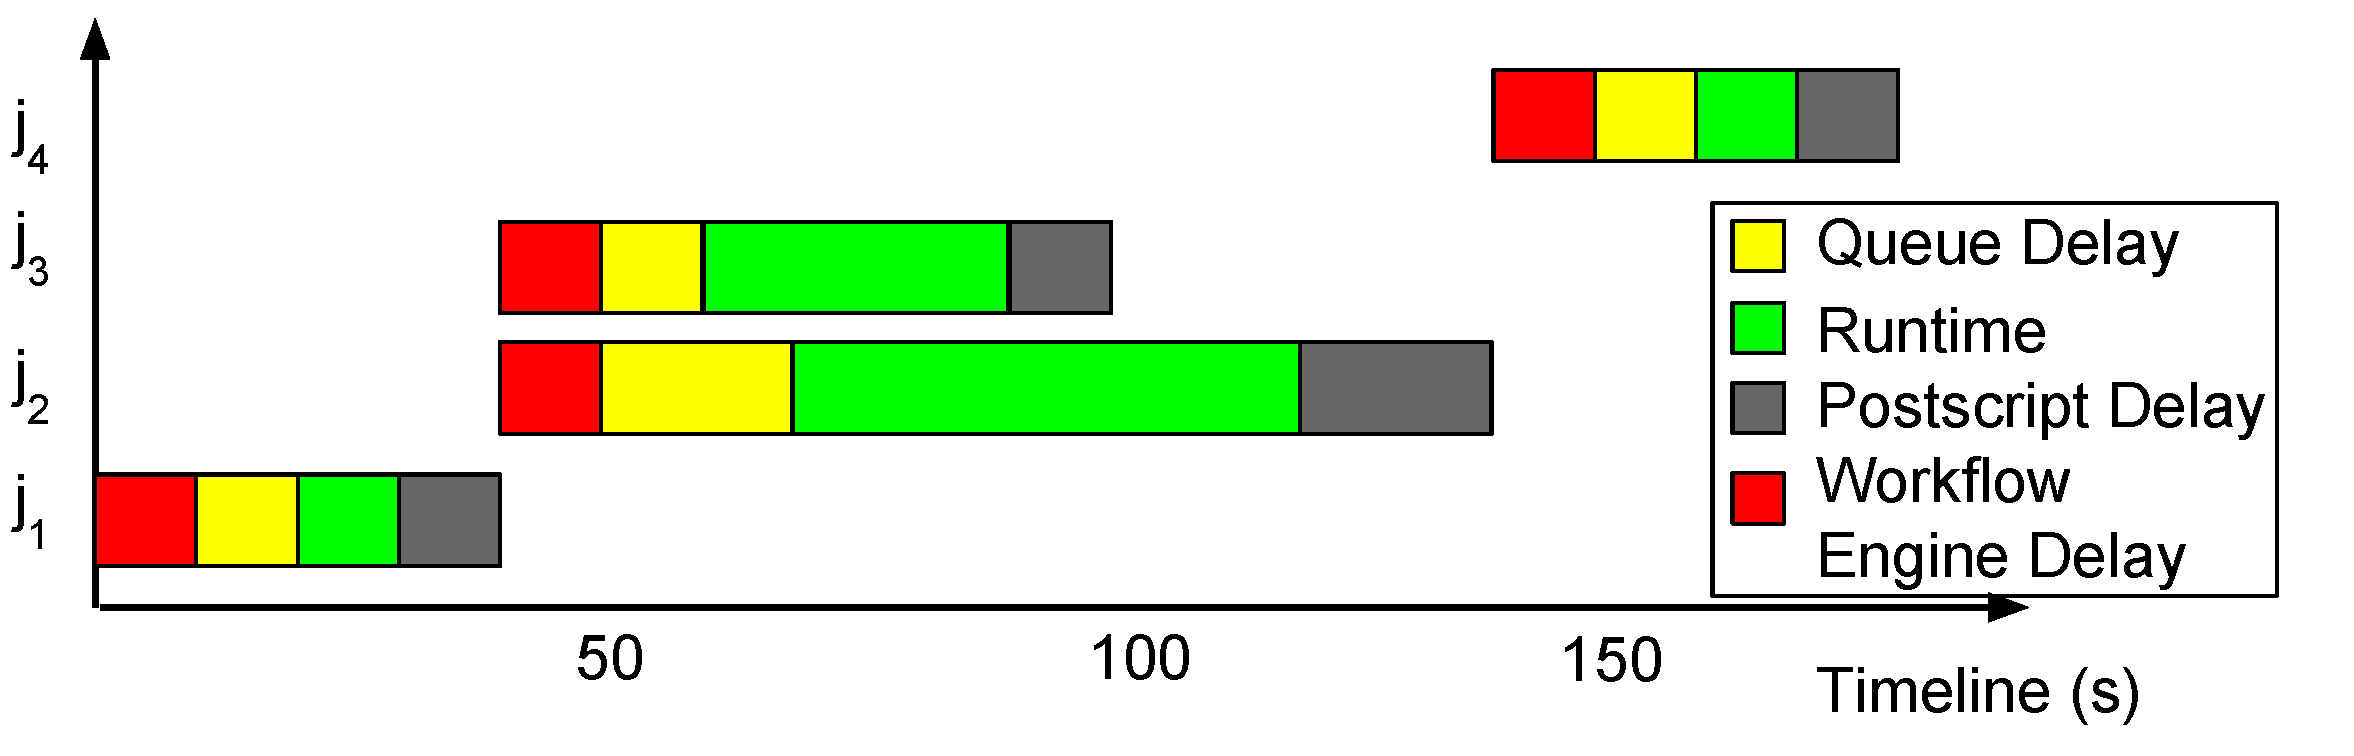
\includegraphics[width=0.7\textwidth]{figures/profiling/overhead_timeline.pdf}
    \caption{Workflow Timeline}
    \label{fig:profiling_overhead_timeline}
\end{figure*}

\begin{figure*}[!htb]
	\centering
 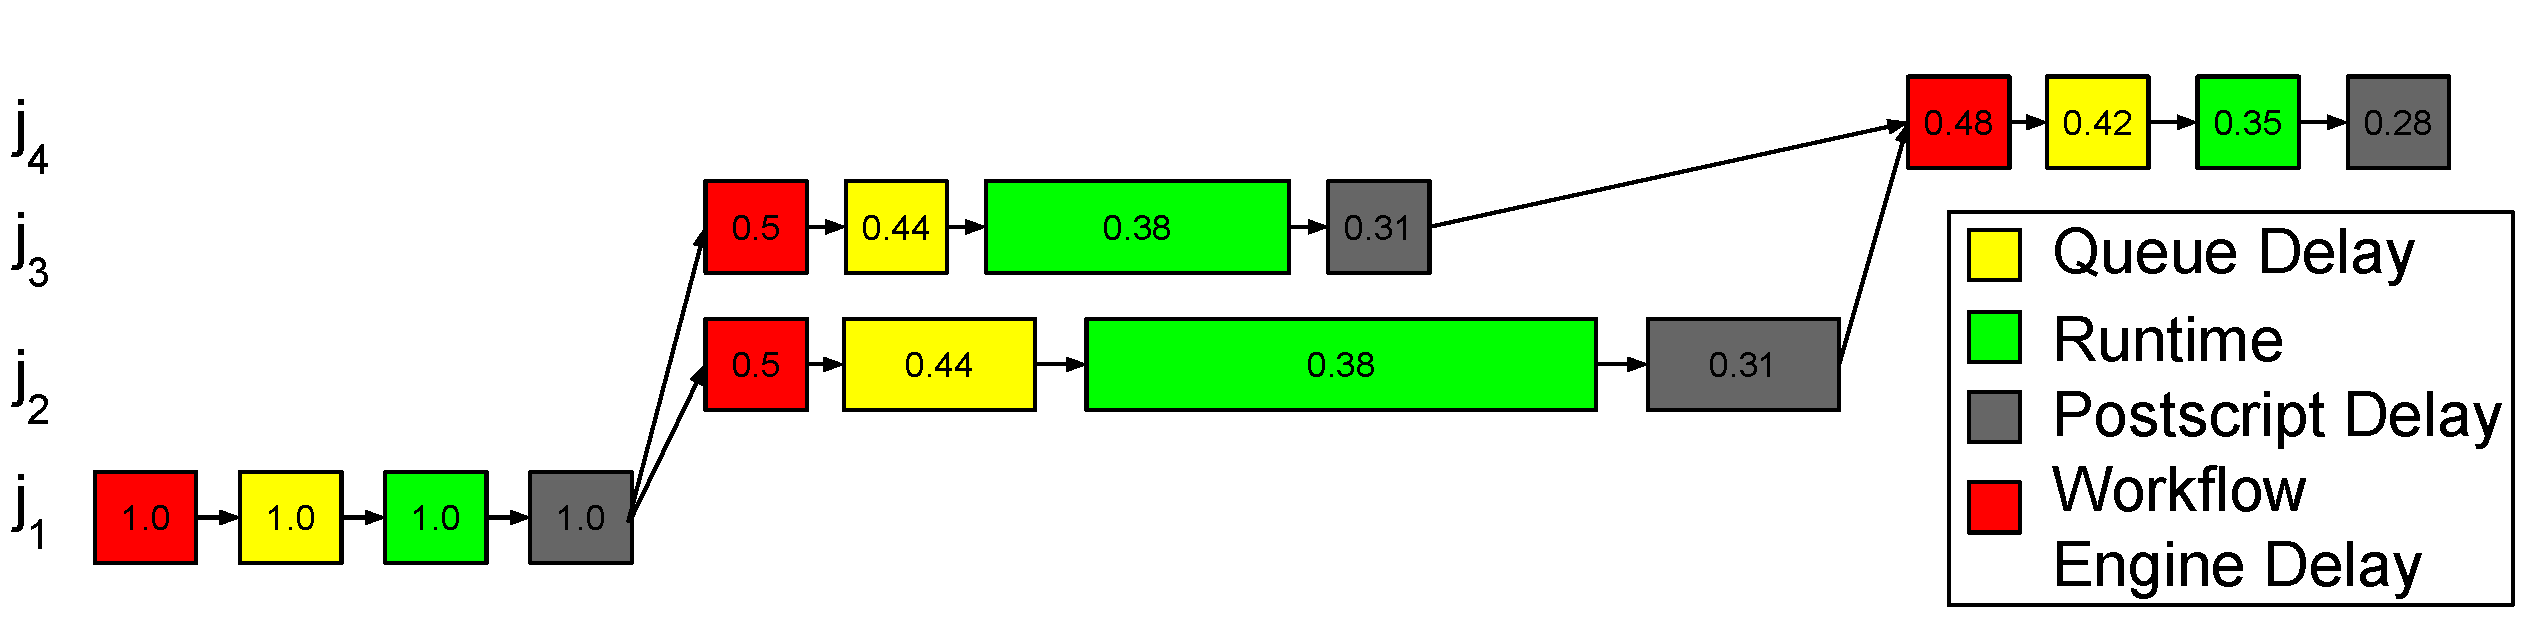
\includegraphics[width=0.8\textwidth]{figures/profiling/rr.pdf}
    \caption{Impact Factor}
    \label{fig:profiling_overhead_rr}
\end{figure*}


\subsection{Metrics to Evaluate Cumulative Overheads and Runtimes}

In this section, we propose four metrics to calculate cumulative overheads of workflows, which are $Sum$, $Projection(PJ)$, $Exclusive~Projection(EP)$ and $Impact~Factor(IF)$. $Sum$ simply adds up the overheads of all jobs without considering their overlap. $PJ$ subtracts from $Sum$ all overlaps of the same type of overhead. It is equal to the projection of all overheads to the timeline. $EP$ subtracts the overlap of all types of overheads from $PJ$. It is equal to the projection of overheads of a particular type excluding all other types of overheads to the timeline. $IF$ uses a reverse ranking algorithm to index overheads and then calculates the cumulative overhead weighted by the ranks (impact factors). The idea is brought by web page indexing algorithms such as PageRank \cite{PageRank1999}. The calculation of $Sum$, $PJ$ and $EP$ is straightforward and Fig.~\ref{fig:profiling_overhead_rr} shows how to calculate the impact factor $(IF)$ of the same workflow graph in Fig.~\ref{fig:profiling_overhead_timeline}. Both $PJ$ and $EP$ are proposed to answer Questions (1) and (2) and $IF$  answers Question (3), while $Sum$ serves as a comparison for them. 

\begin{equation} \label{eq:profiling_rr}
IF(j_u)=d+(1-d)\times\sum_{j_v\in Child(j_u)}{}\frac{IF(j_v)}{||Parent(j_v)||}
\end{equation}

Equation~\ref{eq:profiling_rr} means that the $IF$ of a node (overhead or job runtime) is determined by the $IF$ of its child nodes. $d$ is the damping factor, which controls the speed of the decrease of the $IF$. $||Parent(j_v)||$ is the number of parents that node $j_v$ has. Intuitively speaking, a node is more important if it has more children and/or its children are more important. In terms of workflows, it means an overhead has more power to control the release of other overheads and computational activities. There are two differences compared to the original PageRank:  
\begin{enumerate}
\item We use output link pointing to child nodes while PageRank uses input link from parent nodes, which is why we call it reverse ranking algorithm.
\item Since a workflow is a DAG, we do not need to calculate $IF$ iteratively. For simplicity, we assign the $IF$ of the root node to be 1. And then we calculate the $IF$ of a workflow ($G$) based on the equation below, while $\phi_{j_u}$ indicates the duration of node $j_u$.  

\begin{equation} \label{eq:profiling_sum_rr}
IF(G)=\sum_{}{}IF(j_u) \times \phi_{j_u}
\end{equation}

\end{enumerate}

$IF$ has two important features: (1) $IF$ of a node indicates the importance of this node in the whole workflow graph and its likelihood to be a bottleneck, the greater the more important; (2) $IF$ decreases from the top of the workflow to down, the speed of which is controlled by the damping factor $d$. It reflects the intuition that the overhead occurred at the beginning of the workflow execution is likely to be more important than that at the end.
By analyzing these four types of cumulative overheads, researchers have a clearer view of whether their optimization methods have overlapped the overheads of a same type (if $PJ < Sum$) or other types (if $EP < PJ$). Besides importance, $IF$ is also able to show the connectivity within the workflow, the larger the denser. 
We use a simple example workflow with four jobs to show how to calculate the overlap and cumulative overheads. Fig.~\ref{fig:profiling_overhead_timeline} shows the timeline of our example workflow. $j_1$ and $j_4$ are the parent and children of $j_2$ and $j_3$ respectively.
\begin{table*}[htb!]
\caption{Overhead and Runtime Information}
\label{tab:profiling_stats}
\centering
\begin{tabular}{lrrrrrr}
\hline
Job & Release Time &Queue Delay & Workflow Engine Delay & Runtime &Postscript Delay\\

\hline

$j_1$ & 0 & 10 & 10 & 10 & 10\\ 
$j_2$ & 40 & 10 &20 &50&20\\
$j_3$ &40&10&10&30&10\\
$j_4$ &150&10&10&10&10\\

\hline
\end{tabular}
\end{table*} 


At $t$=0,  $j_1$ is first released and once it is done at $t$=40, $j_3$ and $j_2$ are released. Finally, at $t$=140, $j_4$ is released. Table.~\ref{tab:profiling_stats} shows their overhead and runtime duration (assuming). 
For example, $PJ$ of queue delay is 40 since the queue delay of $j_2$ and $j_3$ overlaps from $t$=50 to 60. $EP$ of queue delay is 10 less than $PJ$ of queue delay since the queue delay of $j_2$ overlaps with the runtime of $j_3$ from $t$=60 to 70. 

For simplicity, we do not include the data transfer delay, prescript delay and others. The overall makespan for this example workflow is 180. Table~\ref{tab:model_percentage_overhead} shows the percentage of overheads and job runtime over makespan.  

\begin{table}[h!]
\caption{Percentage of Overheads and Runtime}
\label{tab:model_percentage_overhead}
\centering
\begin{tabular}{lrrrr}
\hline
Contribution & Sum & PJ & EP &IF\\

\hline

runtime(\%) & 57.1 & 42.8 & 28.5 &17.7 \\
queue delay(\%) & 28.5 &21.4 &14.2 &13.0 \\
workflow engine delay(\%) & 21.4 &14.2& 14.2 &14.2\\
postscript delay(\%) & 28.5 & 28.5 & 21.4 & 11.2 \\
\hline
\end{tabular}
\end{table} 


In Table~\ref{tab:model_percentage_overhead}, we can conclude that the sum of $Sum$ is larger than makespan and smaller than makespan$\times$(number of resources) because it does not count the overlap at all. $PJ$ is larger than makespan since the overlap between more than two types of overheads may be counted twice or more. $EP$ is smaller than makespan since some overlap between more than two types of overheads may not be counted.  $RR$ shows how intensively these overheads and computational activities are connected to each other. 

\subsection{Experiments and Evaluations}

We applied these four metrics to a widely used workflow in our experiments. These workflows were run on distributed platforms including clouds, grids and dedicated clusters. 
On clouds, virtual machines were provisioned and then the required services (such as file transfer services) were deployed. 
We examined two clouds: Amazon EC2 \cite{AmazonEC2}  and FutureGrid \cite{FutureGrid}. Amazon EC2 is a commercial, public cloud that is been widely used in distributed computing. 
We examined the overhead distributions of a widely used astronomy workflow called Montage \cite{Berriman2004} that is used to construct large image mosaics of the sky. Montage was run on FutureGrid \cite{FutureGrid}. FutureGrid is a distributed, high-performance testbed that provides scientists with a set of computing resources to develop parallel, grid, and cloud applications. 
%Should be included in final defense
\subsection{Relationship between Overhead Metrics and Overall Performance}

In this section, we aim to investigate the relationship between the overhead metrics that we proposed and the overall performance of popular workflow restructuring techniques. Among them, task clustering \cite{Singh2008} is a technique that increases the computational granularity of tasks by merging small tasks together into a clustered job, reducing the impact of the queue wait time and also the makespan of the workflow. Data or job throttling \cite{Humphrey2008} limits the amount of parallel data transfer to avoid overloading supporting services such as data servers. Throttling is especially useful for unbalanced workflows in which one task might be idle while waiting for data to arrive. The aim of throttling is to appropriately regulate the rate of data transfers between the workflow tasks via data transfer servers by ways of restricting the data connections, data threads or data transfer jobs. Provisioning tools often deploy pilot jobs as placeholders for the execution of application jobs. Since a placeholder can allow multiple application jobs to execute during its lifetime, some job scheduling overheads can be reduced. 

\subsubsection{How Task Clustering Reduces Overheads}

\begin{table}[htb]
	\footnotesize
	\centering
	\begin{tabular}{l|rrrr}
Metric & Workflow Engine Delay  &Queue Delay& Runtime\\
		\hline
		SUM & $1.5\times 10^5$ & $1.9\times 10^7$ &  $1.5\times 10^6$ \\
		SUM/n & 54(0.16\%) & $6.8\times 10^3$(20\%)& 515(1.6\%) \\
		PJ & $3.2\times 10^3$(9.3\%) & $2.9\times 10^4$(85\%) & $3.3\times 10^4$(102\%) \\
		EP & 70(0.2\%) & 665(1.9\%) & $4.5\times 10^3$(14\%) \\
		IF & 310(0.9\%)& $1.6\times 10^4$(45\%) & $3.1\times 10^3$(9.4\%)\\
	\end{tabular}
		\caption{Metrics Without Task Clustering}
		\label{tab:profiling_no_clustering}
	\quad
	\begin{tabular}{l|rrrr}
Metric & Workflow Engine Delay  &Queue Delay& Runtime\\
		\hline
		SUM & 681(74\%) & $1.0\times 10^3$(112\%) &  $4.4\times 10^3$(475\%) \\
		SUM/n & 6.6(0.72\%) & 10(1.1\%)& 43(4.6\%) \\
		PJ & 116(13\%) & 197(21\%) & 660(72\%) \\
		EP & 72(7.8\%) & 90(9.8\%) & 420(46\%) \\
		IF & 117(13\%)& 165(18\%) & 442(48\%)\\
	\end{tabular}
		\caption{Metrics with Task Clustering}
	\label{tab:profiling_clustering}
\end{table}

In the following sections, we use a Montage workflow to show how different optimization methods improve overall performance. Many workflows are composed of thousands of fine computational granularity tasks. Task clustering is a technique that increases the computational granularity of tasks by merging small jobs together into a clustered job, reducing the impact of the queue wait time and minimizing the makespan of the workflow. Table.~\ref{tab:profiling_clustering} and Table.~\ref{tab:profiling_no_clustering} compare the overheads and runtime of the Montage workflow. $SUM/n$ indicates the average overhead or runtime per job.The percentage is calculated by the cumulative overhead ($PJ$, $EP$ or $IF$) divided by the makespan of workflows. 
In this example, we can see that $PJ$, $EJ$ and $IF$ consistently show that the portion of runtime is increased compared to overheads with task clustering. For example, the $IF$ of queue delay without clustering (45\%) is much larger than the $IF$ of runtime (9.4\%). In the case of task clustering, the $IF$ of runtime (48\%) is much larger than the $IF$ of queue delay (18\%). We can conclude that task clustering improves the runtime performance by reducing the influence of queue delay (more specifically, overlapping). The metric $SUM$ and $SUM/n$, which are usually used in other work, do not provide useful insight for us. 


